\newpage
\chapter{Neuronale Netze}
Tauchen Sie ein, in die wundersame Welt der k"unstlichen Intelligenz. \\
Ich beschreibe hier einen neuralen Netzwerk Simulator, der auch von nicht-technischen Leuten,
einfach zu verstehen ist.
Basierend auf backpropagation'es Lernen f"ur das hier vorgestellte Tool, ist es m"oglich,
Ihren Computer zu trainieren und zu lernen, was Sie von ihm erwarten. \\
Ich m"ochte Ihnen zugleich einen Vorrausblick geben, was uns in naher Zukunft erwartet. \\

\section{Arten von Netzwerken}
Folgende neurale Netzwerke, werde ich hier noch vorstellen:\\
* ein Netzwerk, um die Zahlen 1, 2, und 3 zu erkennen. \\
* ein Netzwerk, um die logische Funktion AND zu verarbeiten. \\
* ein Netzwerk, um die logische Funktion XOE zu verarbeiten. \\

\section{Was sind Neuronale Netzwerke ?}
Expert Definition: \\
Ein neurales Netzwerk ist eine parallel-laufende Informationsstruktur.

\subsection{Künstliches Neuron}
Ein künstliches Neuron bildet die Basis für das Modell der künstlichen neuronalen Netze, ein Modell aus der Neuroinformatik, das durch biologische neuronale Netze motiviert ist. Als konnektionistisches Modell bilden sie in einem Netzwerk aus künstlichen Neuronen ein künstliches neuronales Netz und können so beliebig komplexe Funktionen approximieren, Aufgaben erlernen und Probleme lösen, bei denen eine explizite Modellierung schwierig bis nicht durchzuführen ist. Beispiele sind die Gesichts- und Spracherkennung.\\
\\
Als Modell aus dem biologischen Vorbild der Nervenzelle entstanden, kann es mehrere Eingaben verarbeiten und entsprechend über seine Aktivierung reagieren. Dazu werden die Eingaben gewichtet an eine Ausgabefunktion übergeben, welche die Neuronenaktivierung berechnet. Ihr Verhalten wird ihnen im Allgemeinen durch Einlernen unter Verwendung eines Lernverfahrens gegeben.
\subsection{Biologische Motivation}
Motiviert sind künstliche Neuronen durch die Nervenzellen der Säugetiere, die auf die Aufnahme und Verarbeitung von Signalen spezialisiert sind. Über Synapsen werden Signale elektrisch oder chemisch an andere Nervenzellen oder Effektorzellen (etwa zur Muskelkontraktion) weitergeleitet.\\
Eine Nervenzelle besteht aus dem Zellkörper, Axon und den Dendriten. Dendriten sind kurze Zellfortsätze, die stark verzweigt für die Aufnahme von Signalen anderer Nervenzellen oder Sinneszellen sorgen. Das Axon funktioniert als Signalausgang der Zelle und kann eine Länge bis 1 m erreichen. Der Übergang der Signale erfolgt an den Synapsen, welche erregend oder hemmend wirken können.\\
Die Dendriten der Nervenzelle leiten die eingehenden elektrischen Erregungen an den Zellkörper weiter. Erreicht die Erregung einen gewissen Grenzwert und übersteigt ihn, entlädt sich die Spannung und pflanzt sich über das Axon fort (Alles-oder-nichts-Gesetz).
\\
Die Verschaltung dieser Nervenzellen bildet die Grundlage für die geistige Leistung des Gehirns. Das Zentralnervensystem des Menschen besteht nach Schätzungen aus ${\displaystyle 10^{10}}$ bis ${\displaystyle 10^{12}}$ Nervenzellen, die durchschnittlich 10.000 Verbindungen besitzen – das menschliche Gehirn kann also mehr als 10 14 ${\displaystyle 10^{14}}$ Verbindungen besitzen. Das Aktionspotential im Axon kann sich mit einer Geschwindigkeit bis zu 100 m/s fortpflanzen.\\
\\
Im Vergleich zu Logikgattern zeigt sich auch die Effizienz von Neuronen. Während Gatter im Nanosekunden-Bereich $(10^{-9})$ schalten, unter einem Energieverbrauch von $10^{-6}$ Joule (Daten von 1991), reagieren Nervenzellen im Millisekunden-Bereich $(10^{-3})$ und verbrauchen lediglich eine Energie von $10^{-16}$ Joule. Trotz der augenscheinlich geringeren Werte in der Verarbeitung durch Nervenzellen können rechnergestützte Systeme nicht an die Fähigkeiten biologischer Systeme heranreichen.\\
\begin{figure}[h]
\centering
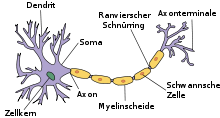
\includegraphics[width=0.7\linewidth]{pics/zelle.png}
\caption[Nervenzelle]{Schema einer Nervenzelle}
\label{fig:zelle}
\end{figure}
Die Vorteile und Eigenschaften von Nervenzellen motivieren das Modell der künstlichen Neuronen. Viele Modelle und Algorithmen zu künstlichen neuronalen Netzen entbehren dennoch einer direkt plausiblen, biologischen Motivierung. Dort findet sich diese nur im Grundgedanken der abstrakten Modellierung der Nervenzelle.

\subsection{Modellierung}
Mit der Biologie als Vorbild wird nun durch eine passende Modellbildung eine für die Informationstechnik verwendbare Lösung gefunden. Durch eine grobe Verallgemeinerung wird das System vereinfacht – unter Erhaltung der wesentlichen Eigenschaften.\\
Die Synapsen der Nervenzelle werden hierbei durch die Addition gewichteter Eingaben abgebildet, die Aktivierung des Zellkerns durch eine Aktivierungsfunktion mit Schwellenwert.

\subsection{Bestandteile}
Ein künstliches Neuron ${\displaystyle j}$ kann durch vier Basiselemente beschrieben werden:
\begin{itemize}
\item[1.] \textbf{Wichtung}: Die Gewichte ${\displaystyle w_{ij}}$ bestimmen den Grad des Einflusses, den die Eingaben des Neurons in der Berechnung der späteren Aktivierung einnehmen. Abhängig von den Vorzeichen der Gewichte kann eine Eingabe hemmend (inhibitorisch) oder erregend (exzitatorisch) wirken. Ein Gewicht von 0 markiert eine nicht existente Verbindung zwischen zwei Knoten.
\item[2.] Übertragungsfunktion: Die Übertragungsfunktion ${\displaystyle \Sigma }$ berechnet anhand der Wichtung der Eingaben die Netzeingabe des Neurons.
\item[3.] Aktivierungsfunktion: Die Ausgabe des Neurons wird schließlich durch die Aktivierungsfunktion ${\displaystyle \varphi }$ bestimmt. Die Aktivierung wird beeinflusst durch die Netzeingabe aus der Übertragungsfunktion sowie einem Schwellenwert.
\begin{figure*}[h]
\centering
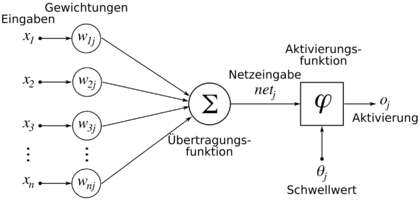
\includegraphics[width=0.7\linewidth]{pics/kneuron.png}
\caption[künstliches Neuron]{Darstellung eines künstlichen Neurons mit seinen Elementen}
\label{fig:kneuron}
\end{figure*}
\item[4.] Schwellenwert: Das Addieren eines Schwellenwerts ${\displaystyle \theta _{j}}$ zur Netzeingabe verschiebt die gewichteten Eingaben. Die Bezeichnung bestimmt sich aus der Verwendung einer Schwellenwertfunktion als Aktivierungsfunktion, bei der das Neuron aktiviert wird, wenn der Schwellenwert überschritten ist. Die biologische Motivierung dabei ist das Schwellenpotential bei Nervenzellen. Mathematisch gesehen wird die Trennebene, die den Merkmalsraum auftrennt, durch einen Schwellenwert mit einer Translation verschoben.
\end{itemize}
Durch einen Verbindungsgraphen werden folgende Elemente festgelegt:
\begin{itemize}
\item[1.] Eingaben: Eingaben ${\displaystyle x_{i}}$ können einerseits aus dem beobachteten Prozess resultieren, dessen Werte dem Neuron übergeben werden, oder wiederum aus den Ausgaben anderer Neuronen stammen. Sie werden auch so dargestellt:
\begin{figure}[h]
\centering
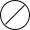
\includegraphics[width=0.5cm, height=0.5cm]{pics/input.png}
\caption[input neuron]{Symbol eines aktivierten Neurons}
\label{fig:input}
\end{figure}
\item[2.] Aktivierung oder Ausgabe: Das Ergebnis der Aktivierungsfunktion wird analog zur Nervenzelle als Aktivierung ${\displaystyle o_{j}}$ des künstlichen Neurons ${\displaystyle j}$ bezeichnet.
\end{itemize}

\section{Mathematische Definition}
Das künstliche Neuron als Modell wird in der Literatur meist auf dem folgenden Weg eingeführt:
Zuerst wird die Netzeingabe\\
\\
${\displaystyle {\mbox{net}}_{j}}$ des künstlichen Neurons ${\displaystyle j}$ durch\\ \\
${\displaystyle {\mbox{net}}_{j}=\sum _{i=1}^{n}x_{i}w_{ij}}$ \\
\\ \\
definiert und damit die Aktivierung \\
\\
${\displaystyle o_{j}}$ durch \\
${\displaystyle o_{j}=\varphi ({\mbox{net}}_{j}-\theta _{j})}$ . \\
\\
Dabei ist\\
${\displaystyle n}$  die Anzahl der Eingaben und \\
${\displaystyle x_{i}}$ die Eingabe ${\displaystyle i}$, die sowohl diskret als auch stetig sein kann. 

\subsection{on-Neuron}
Alternativ kann der Schwellenwert auch durch Hinzufügen eines weiteren Eingangs ${\displaystyle x_{0}}$, einem sogenannten on-Neuron oder auch Bias, dargestellt werden. Dieser hat den konstanten Wert ${\displaystyle x_{0}=1}$. Der Schwellenwert ist dann die Gewichtung dieses Eingangs ${\displaystyle w_{0j}=-\theta _{j}}$. Eine spezielle Behandlung des Schwellenwerts kann so entfallen und vereinfacht die Behandlung in den Lernregeln.\\
\\
Zusätzlich zu den echten Eingängen wird nun der des on-Neurons mit einberechnet:\\
\\
${\displaystyle {\mbox{net}}_{j}=\sum _{i=0}^{n}x_{i} w_{ij}}$\\
\\
\\
Bei der Aktivierung ${\displaystyle o_{j}}$ kann damit auf eine spezielle Behandlung des Schwellenwerts verzichtet werden:\\
\\
${\displaystyle o_{j}=\varphi ({\mbox{net}}_{j})}$ 

\section{Merkmalsraum}
Die Mustererkennung untersucht die automatische Klassifizierung, also wie man Objekte automatisch in Klassen einordnen kann. Um Objekte zu unterscheiden, bestimmt man zunächst eine Reihe von Merkmalen, in denen sie sich möglichst stark unterscheiden. Dann misst man für jedes zu klassifizierende Objekt diese Merkmale und schreibt die Messergebnisse untereinander in einen Vektor, den sogenannten Merkmalsvektor. Man erhält dadurch für jedes Objekt einen Vektor mit so vielen Einträgen, wie Merkmale betrachtet werden. Jeder dieser Vektoren bezeichnet einen Punkt im Merkmalsraum; der Merkmalsraum hat also so viele Dimensionen wie Merkmale betrachtet werden. Gesucht ist nun eine Funktion, die den Merkmalsraum in mehrere Klassen zerlegt, ein sogenannter Klassifikator.

\subsection{Merkmalsvektor}
Ein Merkmalsvektor fasst die (numerisch) parametrisierbaren Eigenschaften eines Musters in vektorieller Weise zusammen. Verschiedene, für das Muster charakteristische Merkmale bilden die verschiedenen Dimensionen dieses Vektors. Die Gesamtheit der möglichen Merkmalsvektoren nennt man den Merkmalsraum. Merkmalsvektoren erleichtern eine automatische Klassifikation, da sie die zu klassifizierenden Eigenschaften stark reduzieren (statt eines kompletten Bildes muss zum Beispiel nur ein Vektor aus 10 Zahlen betrachtet werden). Häufig dienen sie als Eingabe für eine Clusteranalyse.\\
In der Mustererkennung gebräuchliche Merkmalsräume sind mehrdimensionale reelle Vektorräume: ${\mathbb{R}{^d}}$ .
Die Dimension d des Raums entspricht der Anzahl der untersuchten Merkmale und kann sehr groß sein.

\subsection{Musterklassifikation}
In der Musterklassifikation werden Muster anhand von ihren parametrisierbaren Eigenschaften, den Merkmalsvektoren, automatisch klassifiziert. Je besser die Merkmale gewählt wurden und je mehr Trainingsmaterial (also je größer die Stichprobe) vorhanden ist, desto besser gelingt eine Klassifikation. Eine größere Dimension in den Merkmalsvektoren bedeutet dabei einen größeren Bedarf an Trainingsmaterial, also auch einen größeren Trainingsaufwand und eine größere Trainingsdauer. Aber dafür erzielt man auch bessere Klassifikationsraten, also eine bessere Klassifikatorqualität. Eine geringe Anzahl von Dimensionen bedeutet dabei ein schnelleres Training und eine kleinere Stichprobe, aber auch geringere Qualität.

\subsection{Klassifikator}
Ein Klassifikator ist ursprünglich der Bearbeiter eines Sachkatalogs im Bibliothekswesen.[1] Allgemein bezeichnet Klassifikator eine Instanz, die Objekte klassifiziert, d. h. in Kategorien einordnet.\\
\\
Welcher Art eine solche Instanz ist, ist vom betrachteten Szenario abhängig: In der Informatik ist ein Klassifikator häufig ein Algorithmus oder ein Programmobjekt, speziell in der Mustererkennung eine mathematische Funktion, die einen Merkmalsraum auf eine Menge von Klassen abbildet. Auch mechanische Bauteile, zum Beispiel zum Sortieren von Münzen nach Größe, können Klassifikatoren darstellen.\\
\\
In vielen Fällen ist die Unterscheidung zwischen Verfahren und Instanz nicht notwendig oder sinnvoll, weshalb der Begriff Klassifikator häufig gleichbedeutend mit Klassifikationsverfahren verwendet wird.

\subsection{Klassifikationsverfahren}
Klassifikationsverfahren auch Klassifizierungsverfahren sind Methoden und Kriterien zur Einteilung (Klassierung) von Objekten oder Situationen in Klassen, das heißt zur Klassifizierung. Ein solches Verfahren wird auch als Klassifikator bezeichnet. Viele Verfahren lassen sich als Algorithmus implementieren; man spricht dabei auch von maschineller oder automatischer Klassifikation. Klassifikationsverfahren sind immer anwendungsbezogen, so dass viele verschiedene Methoden existieren.\\
Im engen Sinne stehen im Gegensatz zu den Klassifikationsverfahren die Klassierungsverfahren welche dem Einordnen von Objekten in bereits existierende Klassen dienen. Umgangssprachlich wird jedoch zwischen Klassifizieren und Klassieren kein Unterschied gemacht.\\
\\
Klassifikationsverfahren spielen unter anderem bei der Mustererkennung, in der Künstlichen Intelligenz und der Dokumentationswissenschaft beziehungsweise dem Information Retrieval eine Rolle. Zur Beurteilung eines Klassifikators können verschiedene Kenngrößen ermittelt werden.

\subsubsection{Arten von Klassifikationsverfahren}
Da eine streng hierarchische Einteilung von Klassifikationsverfahren kaum möglich ist, lassen sie sich am besten anhand verschiedener Eigenschaften einteilen:
\begin{itemize}
\item Manuelle und automatische Verfahren
\item Numerische und nichtnumerische Verfahren
\item Statistische und verteilungsfreie Verfahren
\item Überwachte und nichtüberwachte Verfahren
\item Fest dimensionierte und lernende Verfahren
\item Parametrische und nichtparametrische Verfahren
\end{itemize}

\subsubsection{Manuelle und automatische Verfahren}
Bei automatischen Verfahren findet die Klassifizierung mittels eines automatischen Prozesses durch Software statt. Der Prozess der maschinellen Klassifikation kann als formale Methode des Entscheidens in neuen Situationen aufgrund erlernter Strukturen bezeichnet werden. Die maschinelle Klassifikation ist ein Teilgebiet des Maschinellen Lernens.\\
\\
Genauer ist dies die Erzeugung eines Algorithmus (der lernende Algorithmus), der - angewandt auf bekannte und schon klassifizierte Fälle (die Datenbasis) - Strukturen berechnet. Diese neu erlernten Strukturen ermöglichen es einem weiteren Algorithmus (der auswertende Algorithmus), einen neuen und bisher unbekannten Fall aufgrund der beobachteten Attribute und deren Ausprägungen einer der bekannten Ziel-Klassen zuzuordnen.

\subsubsection{Statistische und verteilungsfreie Verfahren}
Statistische Verfahren basieren auf Dichteberechnungen und Wahrscheinlichkeiten, während verteilungsfreie Verfahren klare Trennflächen zur Trennung der Klassen benutzen. Die Grenzen zwischen den einzelnen Klassen im Merkmalsraum können durch eine Diskriminanzfunktionen angeben werden.\\
\\
Beispiele für statistische Verfahren sind der Bayes-Klassifikator, der Fuzzy-Pattern-Klassifikator oder Kerndichteschätzer. Die Berechnung von Trennflächen ist durch sogenannte Support-Vector-Maschinen möglich.

\subsubsection{Überwachte und nicht überwachte Verfahren}
Das Erzeugen von Strukturen aus vorhandenen Daten wird auch als Mustererkennung, Diskriminierung oder überwachtes Lernen bezeichnet. Dabei werden Klasseneinteilungen vorgegeben (dies kann auch durch Stichproben geschehen). Im Gegensatz dazu existiert nichtüberwachtes Lernen, bei dem die Klassen der Daten nicht vorgegeben sind, sondern auch diese erlernt werden müssen. Dabei können allerdings beim Bestärkenden Lernen (engl.: reinforcement learning) Informationen hinzukommen, ob eine Klasseneinteilung richtig oder falsch war. Ein Beispiel für unüberwachte Verfahren ist die Clusteranalyse.

\subsubsection{Parametrische und nichtparametrische Verfahren}
Parametrische Verfahren beruhen auf parametrischen Wahrscheinlichkeitsdichten, während nichtparametrischen Verfahren (z.B. Nächste-Nachbarn-Klassifikation) auf lokalen Dichteberechnungen basieren.

\

\chapter{Überwachtes Lernen}
Mit Lernen ist dabei die Fähigkeit gemeint, Gesetzmäßigkeiten nachzubilden.
Die Ergebnisse sind durch Naturgesetze oder Expertenwissen bekannt und werden benutzt,
um das System anzulernen.
\\
Ein Lernalgorithmus versucht, eine Hypothese zu finden, die möglichst zielsichere Voraussagen trifft. Unter Hypothese ist dabei eine Abbildung zu verstehen, die jedem Eingabewert den vermuteten Ausgabewert zuordnet. Dazu verändert der Algorithmus die freien Parameter der gewählten Hypothesenklasse. Oft wird als Hypothesenklasse die Menge aller Hypothesen, die durch ein bestimmtes künstliches neuronales Netzwerk modelliert werden kann, verwendet. In diesem Fall sind die frei wählbaren Parameter die Gewichte der Neuronen. Beim überwachten Lernen werden diese Gewichte derart angepasst, dass die Ausgabe der Neuronen denen eines vorgegebenen Teaching Vectors (engl., Lernvektor) möglichst nahekommt. Die Methode richtet sich also nach einer im Vorhinein festgelegten zu lernenden Ausgabe, deren Ergebnisse bekannt sind. Die Ergebnisse des Lernprozesses können mit den bekannten, richtigen Ergebnissen verglichen, also „überwacht“, werden. \\
\\
Um zu wissen, wann eine Hypothese zielsicher ist, wird ein Fehlermaß eingeführt, das minimiert werden soll. Eine beliebte Wahl ist der mittlere quadratische Fehler aller Trainingsdaten.\\
Ein Lernschritt könnte wie folgt aussehen:\\
\begin{itemize}
\item[1.] Anlegen der Eingabe
\item[2.] Verarbeitung der Eingabe (Propagierung)
\item[3.] Vergleich der Ausgabe mit dem erwünschten Wert (Fehler)
\item[4.] Verkleinern des Fehlers durch Modifikation der Gewichte (z. B. mit Backpropagation)
\end{itemize}
Nach diesem Training bzw. Lernprozess sollte das System in der Lage sein, zu einer unbekannten, den gelernten Beispielen ähnlichen Eingabe, eine korrekte Ausgabe zu liefern.\\
Um diese Fähigkeit zu testen, wird das System validiert. Eine Möglichkeit ist, die verfügbaren Daten in ein Trainingsset und ein Testset zu unterteilen. Das Ziel ist es, das Fehlermaß im Testset, mit dem nicht trainiert wird, zu minimieren. Häufig kommen dafür Kreuzvalidierungsverfahren zur Anwendung.\\
Besitzt das Modell sehr viele Parameter (Gewichte) oder sind nur wenige Trainingsdaten vorhanden, kommt es leicht zur Überanpassung. Das zeigt sich, wenn der Fehler im Trainingsset zwar weiterhin sinkt, aber derjenige im Testset wieder zu steigen beginnt, weil die bekannten Daten einzeln gelernt werden (anstelle der allgemeinen Regel dahinter). Oft wird genau dieser Zeitpunkt abgewartet, um den Trainingsvorgang zu stoppen. Damit wird aber das Testset beim Training verwendet. Zur Beurteilung wird daher ein drittes Validierungsset eingeführt.

\section{Empirische Daten}
Empirie (vom griechischen: empeiría ‚Erfahrung, Erfahrungswissen) ist eine methodisch-systematische Sammlung von Daten. Auch die Erkenntnisse aus empirischen Daten werden manchmal kurz Empirie genannt.

\section{mittlerer quadratische Fehler}
Die mittlere quadratische Abweichung, auch der mittlere quadratische Fehler genannt und MQF oder MSE (aus dem englischen für mean squared error) abgekürzt, ist ein Begriff der mathematischen Statistik. Er gibt in der Schätztheorie an, wie sehr ein Punktschätzer um den zu schätzenden Wert streut. Damit ist er ein zentrales Qualitätskriterium für Schätzer.

\section{Punktschätzer}
Als Punktschätzer bezeichnet man eine Schätzfunktion, die jeder Stichprobe einen Wert zuordnet, der eine gewisse Eigenschaft des zugrundeliegenden Wahrscheinlichkeitsmaßes schätzen soll. In den meisten Anwendungen ist die interessierende Größe ein Parameter der Wahrscheinlichkeitsverteilung der Beobachtungen (wie z.B. der Mittelwert)

\section{Schätzfunktion}
Eine Schätzfunktion dient in der mathematischen Statistik dazu, aufgrund von vorhandenen empirischen Daten einer Stichprobe einen Schätzwert zu ermitteln und dadurch Informationen über unbekannte Parameter einer Grundgesamtheit zu erhalten. Schätzfunktionen sind die Basis zur Berechnung von Punktschätzungen und zur Bestimmung von Konfidenzintervallen mittels Bereichsschätzern und werden als Teststatistiken in Hypothesentests verwendet. Sie sind spezielle Stichprobenfunktionen und können durch Schätzverfahren, z. B. die Methode der kleinsten Quadrate  bestimmt werden.\\
Im Rahmen der Entscheidungstheorie können Schätzfunktionen auch als Entscheidungsfunktionen bei Entscheidungen unter Unsicherheit betrachtet werden.

\section{Grundgesamtheit}
Bezeichnet zum Beispiel die Gesamtheit von Populationen.
Die Menge aller Einheiten (auch Merkmalsträger, Untersuchungseinheit) mit übereinstimmenden Identifikationskriterien
(sachlich, räumlich und zeitgleich). \\
Die Einheit ist Träger der Informationen für die Untersuchung

\section{Stickprobe}
Als Stichprobe bezeichnet man eine Teilmenge einer Grundgesamtheit, die unter bestimmten Gesichtspunkten ausgewählt wurde.
\subsection{Auswahlverfahren}
Ein Auswahlverfahren ist die Art und Weise, wie die Elemente der Stichprobe möglichst zweckmäßig ausgewählt werden. Es gibt verschiedene Auswahlverfahren, die nachfolgend beschrieben werden.
\subsubsection{Zufallsauswahl}
Eine Zufallsstichprobe ist notwendig, wenn die Stichprobe repräsentativ sein soll, d. h. wenn von ihr nach dem Induktionsprinzip auf die Grundgesamtheit geschlossen werden soll, da es oft nicht möglich ist, die Grundgesamtheit (etwa die Gesamtbevölkerung oder alle Exemplare eines bestimmten Produkts) zu untersuchen.
\subsubsection{Bewusste Auswahl}
Bei einer systematischen Stichprobenziehung werden bereits bekannte Informationen über die auszuwählenden Fälle genutzt. Die Auswahl erfolgt anhand von Listen und festgelegten Regeln. Mathematisch-statistische Modelle, etwa die Berechnung der Einschlusswahrscheinlichkeit, sind bei bewussten Auswahlen nicht anwendbar. Systematische Auswahlverfahren kommen zum Beispiel im kommerziellen Bereich vor, wenn es auf Repräsentativität nicht ankommt.
\subsubsection{Willkürliche Auswahl}
Bei willkürlichen Stichproben werden Elemente aus der Grundgesamtheit (etwa von einem Interviewer) mehr oder weniger willkürlich in die Stichprobe aufgenommen. Die Auswahl liegt im Ermessen des Interviewers.

\section{Systematische Stischprobe}
Als Systematische Stichprobe (auch Bewusste Auswahl) bezeichnet man Auswahlverfahren, bei denen subjektive Erwägungen die Auswahl der Zielpersonen bestimmen.\\
\\
\textbf{Beispiel}: Alle Mitarbeiter mit mehr als 10 Jahren Betriebszugehörigkeit.\\
\\
Es werden Vorinformationen über die auszuwählenden Fälle genutzt. Verallgemeinerungen sind auf der Basis mathematisch-statistischer Modelle bei bewussten Auswahlen nicht möglich.

\section{Stichprobenvariable}
An dieser Stelle setzt die statistische Modellierung an. Die Stichprobenvariable ${\displaystyle X_{i}}$, eine Zufallsvariable, beschreibt mit ihrer Verteilung die Wahrscheinlichkeit, mit der eine bestimmte Merkmalsausprägung bei der i ${\displaystyle i}$ Ziehung aus der Grundgesamtheit auftritt. Jeder Beobachtungswert ${\displaystyle x_{i}}$ ist die Realisierung einer Stichprobenvariable ${\displaystyle X_{i}}$.

\section{Stichprobenfunktion}
Die Definition von Stichprobenvariablen ${\displaystyle X_{i}}$ erlaubt die Definition von Stichprobenfunktionen analog z. B. zu Kennwerten aus der deskriptiven Statistik:
\subsection{Arithmetisches Mittel - Formel}
{\Large{$\bar{\mathrm{x}} = \frac{x_1 + \ldots + x_n}{n}$}}
\subsection{Stichprobenfunktion - Formel}
{\Large{$\bar{\mathrm{X}} = \frac{X_1 + \ldots + X_n}{n}$}}

\section{Stichprobenverteilung}
Unter Stichprobenverteilung versteht man die Verteilung einer Stichprobenfunktion ${\displaystyle g(X_{1},\dotsc ,X_{n})}$ über alle möglichen Stichproben aus der Grundgesamtheit. Die Stichprobenfunktion ${\displaystyle g}$ ist in der Regel eine Schätzfunktion für einen unbekannten Parameter der Grundgesamtheit oder eine Teststatistik für eine Hypothese über einen unbekannten Parameter der Grundgesamtheit. Daher spricht man statt von Stichprobenverteilung auch einfach von der Verteilung einer Schätzfunktion oder Teststatistik. Die Verteilung der Stichprobenfunktion dient der Gewinnung von Aussagen über unbekannte Parameter in der Grundgesamtheit aufgrund einer Stichprobe.

\section{Hypothese}
In der Statistik bezeichnet man mit Hypothese eine Annahme, die mit Methoden der mathematischen Statistik auf Basis empirischer Daten geprüft wird. Man unterscheidet als Gegensatzpaar Nullhypothese und Alternativhypothese (auch Gegenhypothese). Häufig sagt die Nullhypothese aus, dass kein Effekt bzw. Unterschied vorliegt oder dass ein bestimmter Zusammenhang nicht besteht. Diese These soll verworfen werden, so dass die Alternativhypothese als Möglichkeit übrig bleibt. Durch dieses indirekte Vorgehen soll die Wahrscheinlichkeit für eine irrtümliche Verwerfung der Nullhypothese kontrolliert klein bleiben. Oft entsteht jedoch Verwirrung beim Anwender, weil dieses Vorgehen die Möglichkeit nahelegt, dass – sofern die Nullhypothese nicht verworfen und die Alternativhypothese damit nicht angenommen werden kann – die Nullhypothese als erwiesen gilt. Dies ist allerdings nicht der Fall.
\subsection{Alternativhypothese}
Als Alternativhypothese ${\displaystyle H_{1}}$ oder ${\displaystyle H_{A}}$ bezeichnet man in der empirischen Wissenschaft häufig eine durch Beobachtungen oder Überlegungen begründete Annahme oder Vermutung, die zur Erklärung bestimmter Phänomene dient und die einer möglicherweise verbreiteten Annahme oder Vermutung (nämlich der Nullhypothese) entgegensteht. Insofern kann die Alternativhypothese als innovativ betrachtet werden.\\
\\
Formal zerlegen die Null- und Alternativhypothese einen Parameterraum ${\displaystyle \Theta }$ in zwei disjunkte nicht leere Teilmengen ${\displaystyle \Theta _{0}}$ und ${\displaystyle \Theta _{1}}$. Die Nullhypothese beinhaltet die Aussage, dass der unbekannte Parameter ${\displaystyle \theta }$ aus ${\displaystyle \Theta _{0}}$ stammt, und die Alternativhypothese, dass der unbekannte Parameter ${\displaystyle \theta }$ aus ${\displaystyle \Theta _{1}}$ stammt.
\\
${\displaystyle H_{0}\colon \theta \in \Theta _{0}}$ vs. \\
${\displaystyle H_{1}\colon \theta \in \Theta _{1}}$  

\section{Teststatistik}
Als Teststatistik (synonyme Begriffe: Testgröße, Prüfgröße, Prüffunktion) bezeichnet man eine bestimmte Stichprobenfunktion, die bei einem Hypothesentest dazu verwendet wird, die Testentscheidung - also Ablehnen oder Nichtablehnen der Nullhypothese - zu treffen.\\
Als Prüfwert wird die Realisation einer Teststatistik anhand einer Stichprobe bezeichnet.
\subsection{Statistische Signifikanz}
Statistisch signifikant wird das Ergebnis eines statistischen Tests genannt, wenn Stichprobendaten so stark von einer vorher festgelegten Annahme (der Nullhypothese) abweichen, dass diese Annahme nach einer vorher festgelegten Regel verworfen wird.
\subsection{Verwendung bei festem Signifikanzniveau}
Vor der Durchführung des Tests, das heißt auch vor der Ziehung der hierzu benötigten Stichprobe, ist die Teststatistik
$\boldsymbol{T}$ eine Zufallsvariable. deren deren Wahrscheinlichkeitsverteilung von jener der Stichprobenvariablen
${X_1, X_2, ... , Xn}$
abhängt, wobei n der Stichprobenumfang ist.
Unter der Annahme, dass die Nullhypothese $(H_0)$ richtig ist, 
wird für die Verteilung der Teststatistik je nach Testverfahren ein bestimmtes Verteilungsmodell angenommen, dessen Verteilungsparameter sich aus der Nullhypothese ergeben. Anhand dieser angenommenen Verteilung sowie des zuvor festgelegten Signifikanzniveaus wird zugleich der Ablehnbereich bestimmt. Nun wird die Stichprobe gezogen und aus den sich dabei ergebenden Stichprobenwerten dem konkrete Wert ${\displaystyle t}$ der Teststatistik errechnet.\\
Zur Ablehnung der Nullhypothese kommt es genau dann, wenn ${\displaystyle t}$ in den Ablehnbereich fällt; anderenfalls wird unter dem verwendeten Signifikanzniveau die Nullhypothese beibehalten. Wenn nämlich die Nullhypothese gilt und damit die unterstellte Verteilung der Teststatistik als richtig angenommen werden kann, entspricht die Wahrscheinlichkeit, dass die Testgröße in den Ablehnbereich fällt und somit die Nullhypothese fälschlich abgelehnt wird (sogenannter Fehler 1. Art), genau dem festgelegten Signifikanzniveau. Das Fallen der Testgröße in den Ablehnbereich ist gleichbedeutend mit der (je nach Testproblem) Über- bzw. Unterschreitung eines bestimmten Schwellenwertes, der auch als ,,Kritischer Wert'' bezeichnet wird.
\subsection{Fehler 1. Art}
Der Fehler 1. Art oder $\alpha$-Fehler (Alpha-Fehler) ist ein Fachbegriff der Statistik.
Er bezieht sich auf eine Methode der mathematischen Statistik, den sogenannten Hypothesentest. Beim Test einer Hypothese liegt ein Fehler 1. Art vor, wenn die Nullhypothese zurückgewiesen wird, obwohl sie in Wirklichkeit wahr ist (beruhend auf falsch positiven Ergebnissen).\\
Die Ausgangshypothese ${\displaystyle H_{0}}$ (Nullhypothese) ist hierbei die Annahme, die Testsituation befinde sich im „Normalzustand“. Wird also dieser "Normalzustand" nicht erkannt, obwohl er tatsächlich vorliegt, ergibt sich ein Fehler 1. Art. Beispiele für einen Fehler 1. Art sind:
    \begin{itemize}
    \item der Patient wird als krank angesehen, obwohl er in Wirklichkeit gesund ist (Nullhypothese: der Patient ist gesund),
    \item der Angeklagte wird als schuldig verurteilt, obwohl er in Wirklichkeit unschuldig ist (Nullhypothese: der Angeklagte ist unschuldig),
    \item der Person wird kein Zugang gewährt, obwohl sie eine Zugangsberechtigung hat (Nullhypothese: die Person hat Zugangsberechtigung)
    \end{itemize}

Die vor einem Test bzw. einer Untersuchung festgelegte maximale Wahrscheinlichkeit, bei einer auf dem Ergebnis des Tests fußenden Entscheidung einen solchen Fehler 1. Art zu begehen (Risiko 1. Art), nennt man auch Signifikanzniveau oder Irrtumswahrscheinlichkeit. In der Regel wählt man ein Signifikanzniveau von 5 $\%$ (signifikant) oder 1 $\%$ (sehr signifikant).

Die andere mögliche Fehlentscheidung, nämlich die Alternativhypothese ${\displaystyle H_{1}}$ zurückzuweisen, obwohl sie wahr ist, heißt Fehler 2. Art.\\

\begin{table}[h!]
\begin{tabular}[t]{| p{4cm} | p{4cm} | p{4cm} |}
\hline \rule[3ex]{0pt}{5.5ex}  & \textbf{Wahrer Sachverhalt: $H_0$
(Es gibt keinen Unterschied)}  & \textbf{Wahrer Sachverhalt: $H_1$
(Es gibt einen Unterschied)} \\ 
\hline \rule[3ex]{0pt}{5.5ex} durch einen statistischen Test fällt eine Entscheidung für: $H_0$ & richtige Entscheidung (Spezifität)
Wahrscheinlichkeit: 1-$\alpha$ & Fehler 2. Art
Wahrscheinlichkeit: $\beta$ \\ 
\hline \rule[3ex]{0pt}{5.5ex} durch einen statistischen Test fällt eine Entscheidung für: $H_1$ & Fehler 1. Art
Wahrscheinlichkeit: $\alpha$ & richtige Entscheidung (Sensitivität)
Wahrscheinlichkeit: 1-$\beta$ \\ 
\hline 
\end{tabular}
\end{table}

\chapter{Aktivierungsfunktionen}
Als Aktivierungsfunktion ${\displaystyle \varphi }$ können verschiedene Funktionstypen verwendet werden, abhängig von der verwendeten Netztopologie. Eine solche Funktion kann nicht-linear, zum Beispiel sigmoid, stückweise linear oder eine Sprungfunktion sein. Im Allgemeinen sind Aktivierungsfunktionen monoton steigend.\\
\\
Lineare Aktivierungsfunktionen unterliegen einer starken Beschränkung, da eine Komposition linearer Funktionen durch arithmetische Umformungen durch eine einzige lineare Funktion dargestellt werden kann. Für mehrschichtige Verbindungsnetzwerke sind sie deswegen nicht geeignet und finden so nur in einfachen Modellen Anwendung.\\
\\
Beispiele für grundlegende Aktivierungsfunktionen sind:\\
\section{Schwellwertfunktion}
Die Schwellenwertfunktion (engl. hard limit), wie sie im Folgenden definiert ist, nimmt nur die Werte
${\displaystyle 0}$ und
${\displaystyle 1}$ an. Den Wert 1 für die Eingabe
${\displaystyle v\geq 0}$, sonst 
${\displaystyle 0}$. Bei subtraktiver Verwendung eines Schwellenwerts
${\displaystyle \theta }$ wird die Funktion nur aktiviert, wenn die zusätzliche Eingabe den Schwellenwert übersteigt. Ein Neuron mit einer solchen Funktion wird auch McCulloch-Pitts-Zelle genannt. Sie spiegelt die Alles-oder-nichts-Eigenschaft des Modells wider.\\
\\
${\displaystyle \varphi ^{\mbox{hlim}}(v)={\begin{cases}1&{\mbox{wenn }}v\geq 0\\0&{\mbox{wenn }}v<0\end{cases}}}$ 

\section{Stückweise lineare Funktion}
Die hier verwendete stückweise lineare Funktion (engl. piecewise linear) bildet ein begrenztes Intervall linear ab, die äußeren Intervalle werden auf einen konstanten Wert abgebildet:\\
\\
${\displaystyle \varphi ^{\mbox{pwl}}(v)={\begin{cases}1&{\mbox{wenn }}v\geq {\frac {1}{2}}\\v+{\frac {1}{2}}&{\mbox{wenn }}-{\frac {1}{2}}<v<{\frac {1}{2}}\\0&{\mbox{wenn }}v\leq -{\frac {1}{2}}\end{cases}}}$

\section{Sigmoid Funktion}
Eine Sigmoidfunktion, Schwanenhalsfunktion oder S-Funktion ist eine mathematische Funktion mit einem
S-förmigen Graphen.
Oft wird der Begriff Sigmoidfunktion auf den Spezialfall logistische Funktion bezogen,
die durch die Gleichung:\\
{\Large{$sig(t) = \frac{1}{1+e^{-t}} = \frac{e^t}{1 + e^t} = \frac{1}{2}*(1 + \tanh \frac{t}{2})$}}\\
\\
${\displaystyle \varphi _{a}^{\mbox{sig}}(v)={\frac {1}{1+\exp(-av)}}.}$ \\ 
\\
Die Werte der obigen Funktionen liegen im Intervall ${\displaystyle [0,1]}$. Für das Intervall ${\displaystyle [-1,+1]}$ lassen sich diese Funktionen entsprechend definieren.

\begin{figure}[h!]
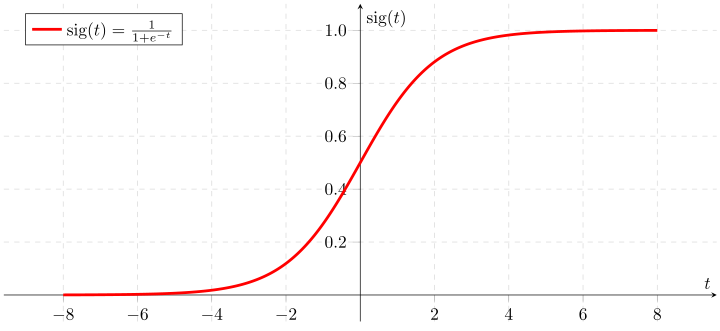
\includegraphics[width=0.7\linewidth]{pics/Sigmoid}
\caption{Graph der Sigmoid-Funktion}
\label{fig:Sigmoid}
\end{figure}

\section{Darstellung boolescher Funktionen}
\MyHeadBottom



Mit künstlichen Neuronen lassen sich boolesche Funktionen darstellen. So können die drei Funktionen Konjunktion (and), Disjunktion (or) und Negation (not) unter Verwendung einer Schwellenwertfunktion ${\displaystyle \varphi ^{\mbox{hlim}}}$ wie folgt repräsentiert werden:\\

\begin{tabular}{| p{4cm} | p{4cm} | p{4cm} |}
\hline \rule[-2ex]{0pt}{5.5ex} \textbf{Konjunktion} & \textbf{Disjunktion} & \textbf{Negation} \\ 
\hline \rule[-2ex]{0pt}{5.5ex}
\begin{minipage}{-1.5\textwidth}
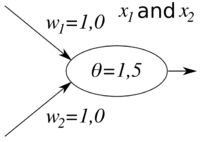
\includegraphics[width=3.5cm]{pics/200px-Und-Neuron.png}
\label{fig:200px-Und-Neuron}
\end{minipage}


Neuron, das die Konjunktion repräsentiert
&
\begin{minipage}{-0.8\textwidth}
\centering
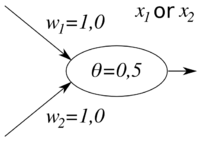
\includegraphics[width=3.5cm]{pics/200px-Oder-Neuron.png}
\label{fig:200px-Oder-Neuron}
\end{minipage}

Neuron, das die Disjunktion repräsentiert
&
\begin{minipage}{-0.8\textwidth}
\centering
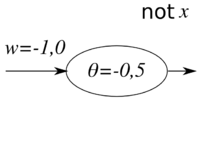
\includegraphics[width=3.5cm]{pics/Nicht-Neuron.png}
\label{fig:Nicht-Neuron}
\end{minipage}

Neuron, das die Negation repräsentiert
\\ 
\hline 
\end{tabular} 